\cleardoublepage
\chapter{Basics}
\label{ch:1}

%------------------------------------------------

\section{Signal Flow and Wiring}

\begin{fullwidth}
Wiring Operators is the most basic operation in TouchDesigner. All projects are made up of nothing more than groups of Operators wired together. Each Operator, on its own, does a very specific thing, but when they are combined together into a 'Network', they can solve extremely complex problems.

All data in TouchDesigner flows from left to right. Any inputs that an Operator has will always be on the left side, and outputs will be on the right side. The inputs and outputs will also be ordered first to last, going from top to bottom. In the example diagram below, follow the two signals starting on the left. As they flow from left to right, they are composited, one over the other.

\begin{center} 
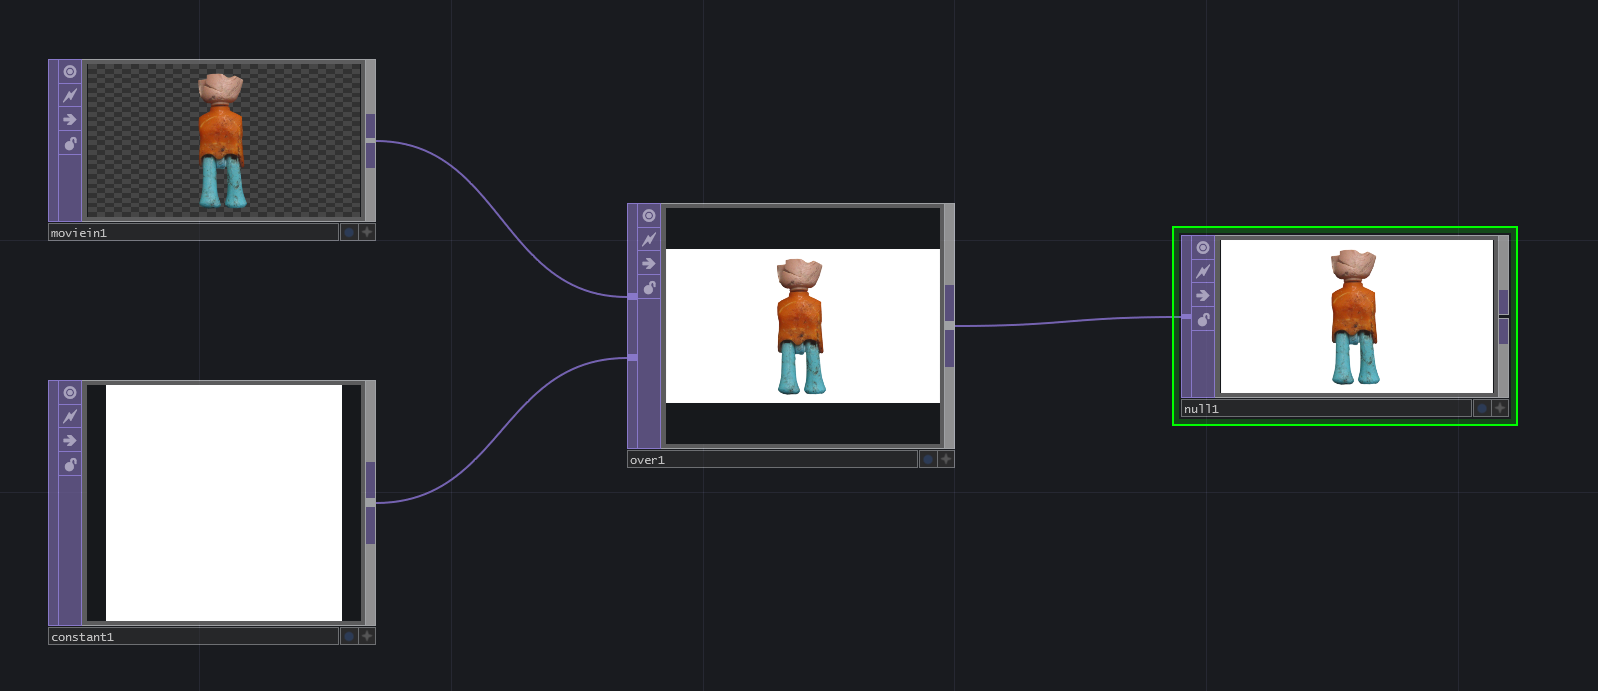
\includegraphics{./img/1.1/signal-flow-1.png}
\end{center}

Components, interestingly, have the same data signal flow as Operators, flowing from left to right, but they are also capable of parent and child relationships, which flow from top to bottom. The component at the top of the signal chain is the parent, and the components below it are its children, and below that are the children's children, and so on. In the example below, there is a small UI, that is made of a few sliders. In this example, the Slider COMPs are the children of the Container COMP, which is the parent.

\begin{center} 
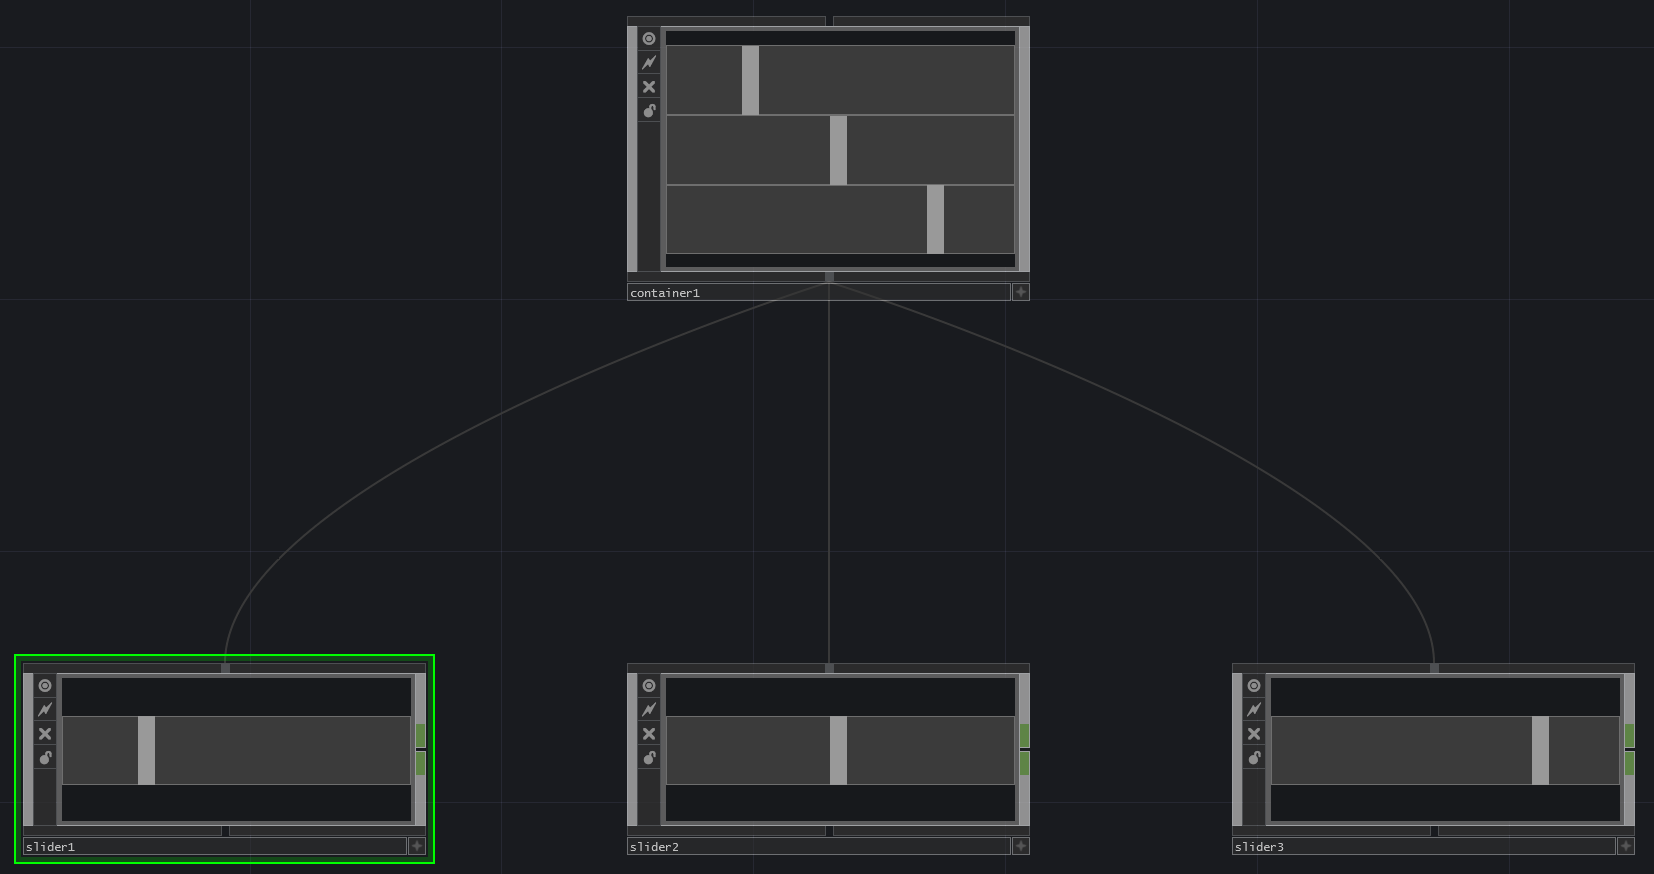
\includegraphics{./img/1.1/signal-flow-2.png}
\end{center}

\end{fullwidth}

%------------------------------------------------

\section{Creating Operators}
\begin{fullwidth}
The OP Create Dialog can be reached in a multitude of ways. Each has a correct time and place of usage. When creating Operators from scratch the two easiest methods are to hit 'Tab' on the keyboard, or to double click on the Network background.

When working with existing chains of Operators, there are two easy ways to add Operators. The first is to right click on either the input or output of an Operator. This will add the chosen Operator, pre-wired, directly before the input or after the output. This is especially useful as it inserts the Operator seamlessly into a pre-existing chain.

For example, there is a Constant TOP wired to a Null TOP, and a Transform TOP needs to be added between the two. Right clicking either the output of the Constant TOP, or the input of the Null TOP, and selecting Transform TOP, would create a Transform TOP, that would be pre-wired in-between the Constant TOP and Null TOP.

The second way to add an Operator to an existing chain is to middle click on the output of an Operator.  The difference is that right clicking integrates the newly created Operator into the current Operator chain, whereas middle clicking creates a new branch in parallel to the chain of Operators.

Similar results can be achieved by right clicking on the wire itself and clicking on 'Insert Operator' or 'Add Operator'.  'Insert Operator' acts like right clicking an Operator's output and integrates it into the current Operator chain, whereas 'Add Operator' acts like middle clicking and creates a new branch in parallel to the chain.

In the diagram below, there is an example with a Constant TOP and a Null TOP. In the next diagram, the wire connecting them was right clicked and a Transform TOP was created using 'Insert Operator'. In the proceeding diagram, the wire connecting the Operators was right clicked and a Transform TOP was created using 'Add Operator'. Notice how it is pre-wired in parallel to the first Transform TOP.


\begin{center} 
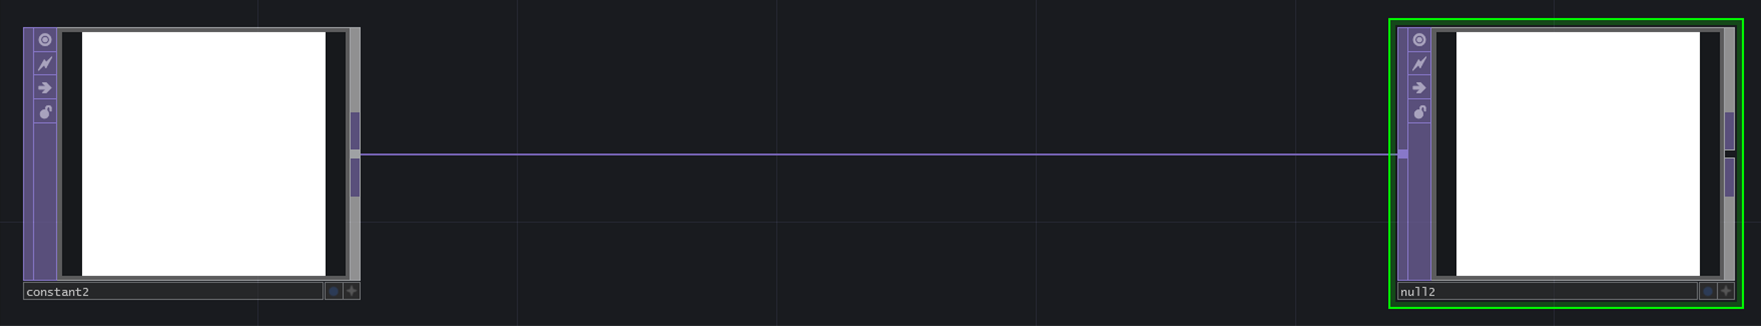
\includegraphics{./img/1.2/creating-operators-1.png}

\center 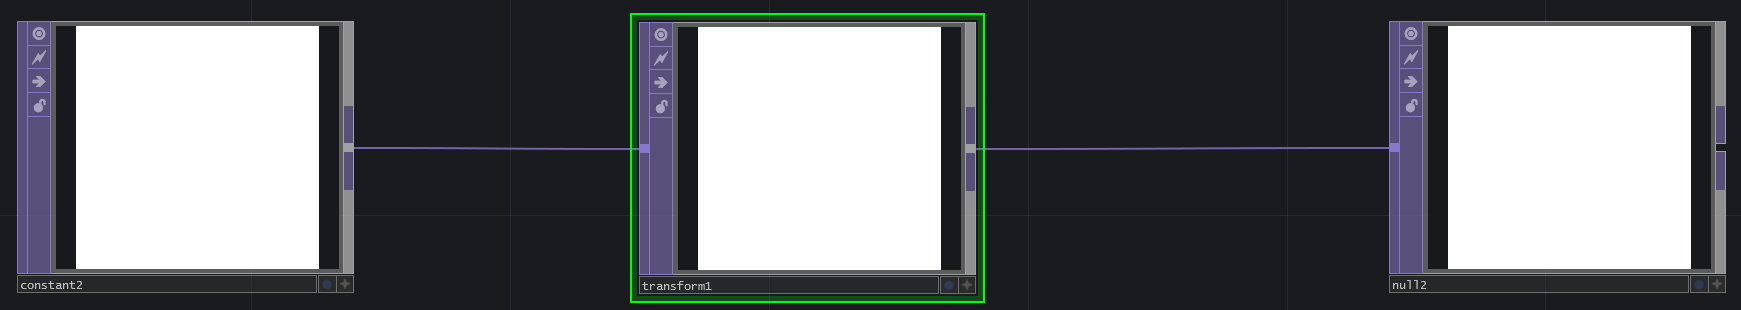
\includegraphics{./img/1.2/creating-operators-2.png}

\center 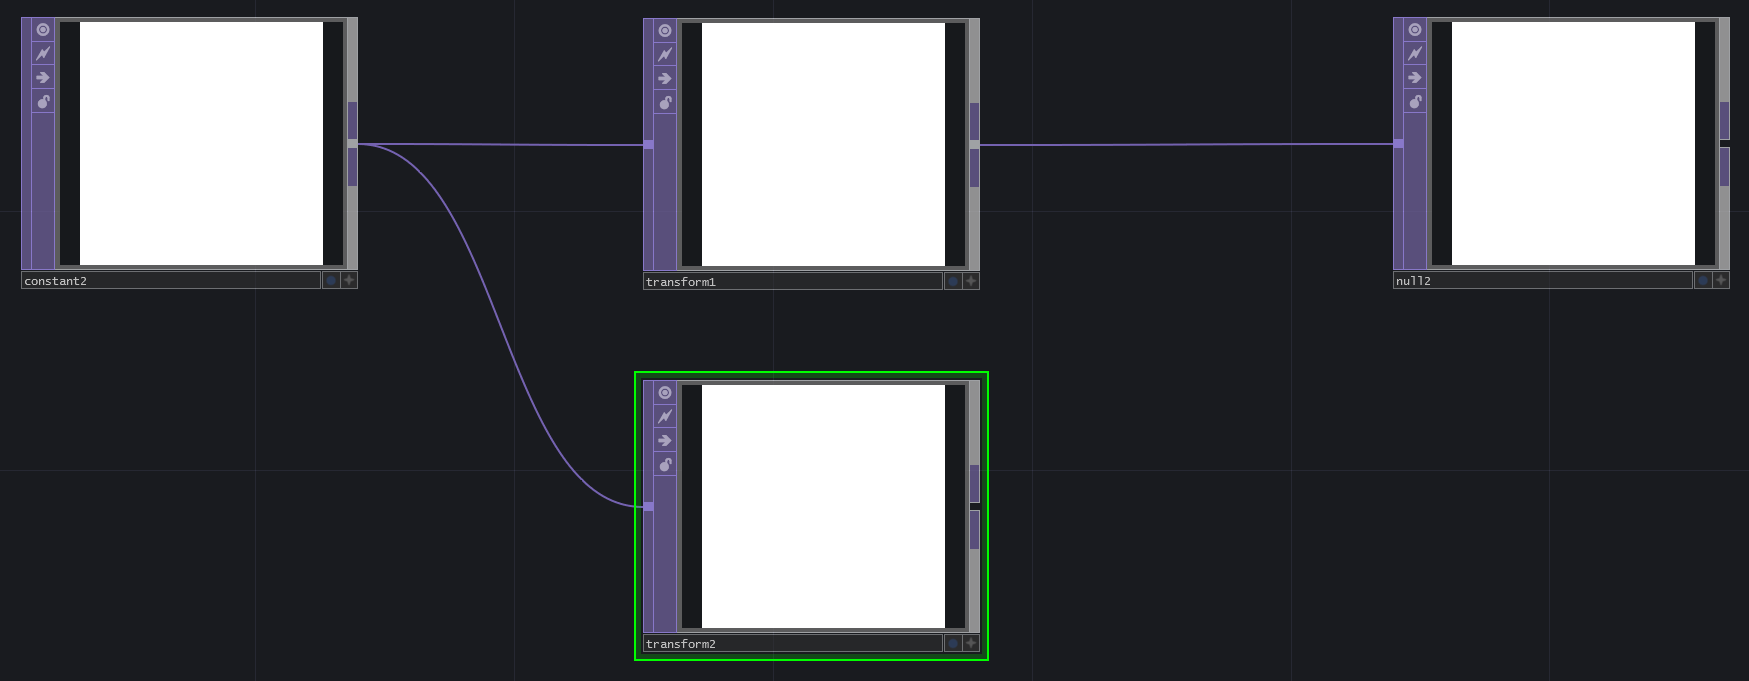
\includegraphics{./img/1.2/creating-operators-3.png}
\end{center}

There are two useful key commands when working with the OP Create Dialog: 'Control' and 'Shift'. Open the OP Create dialog, hold down 'Control' on the keyboard, and then begin to select multiple Operators in a row. Each one will be added to the Network below the last. This is useful for quickly populating a Network with a few different Operators. 

Similarly, open the OP Create dialog, press and hold the 'Shift' key, and then begin to select multiple Operators. This is different than above, in that the Operators will be wired together in series. This key command can be used to quickly create small, or large, chains of pre-wired Operators. 

Both of these key commands are quite powerful, but they become even more so when they are used in tandem. For example, a project requires 3 chains of Operators. The first will consist of a Circle TOP, connected to a Blur TOP, connected to a Null TOP. The second will consist of a Circle TOP, connected to an Edge TOP, connected to a Noise TOP, connected to a Null TOP. The final chain will consist of a Movie In TOP, connected to a Blur TOP, connected to a Null TOP. Let's go through this step by step, to demonstrate practical use of the above key commands:

\begin{enumerate}
\item Open the OP Create dialog
\item Press and hold down 'Shift'
\item While holding 'Shift', click on Circle TOP, Blur TOP, then Null TOP. This will create the first chain.
\item Release the 'Shift' key 
\item Press and hold down 'Control'. This will place the next Operator below the first Operator.
\item Holding 'Control', click on Circle TOP
\item Release the 'Control' key
\item Press and hold down the 'Shift' key
\item While holding 'Shift', click on Edge TOP, Noise TOP, and then Null TOP. This will create the second chain 
\item Release the 'Shift' key
\item Press and hold 'Control'
\item While holding 'Control', click on Movie In TOP. 
\item Release the 'Control' key
\item Press and hold 'Shift' 
\item Click on the remaining operators: Blur TOP, and Null TOP
\item Now that all of the Operators are created, use the 'Esc' key to close the OP Create dialog.
\end{enumerate}

After closing the OP Create Dialog, all the required Operators will be wired and ready to go in the project. These key commands have not only saved having to open and close the OP Create Dialog for every Operator, but they've saved the need to manually wire them.

\end{fullwidth}

%------------------------------------------------

\section{Mouse and Keyboard Navigation}
\begin{fullwidth}
The mouse plays a vital role in TouchDesigner programming, and a high-quality mouse is highly recommended. The mouse is used to move around the Network and work with Operators. 

To navigate around the Network, left click and drag the Network background. Left click on an Operator to select it. Left click and drag that Operator to move it around the Network. Right click on an Operator to reveal a menu with options that will be introduced slowly. To select and work with more than one Operator, right click and drag the selection box around the desired Operators. Middle click on an Operator to get more info about it. There is a UI button that displays the same Operator info window, which is useful when using a mouse that doesn't have a middle click button.

\begin{center}
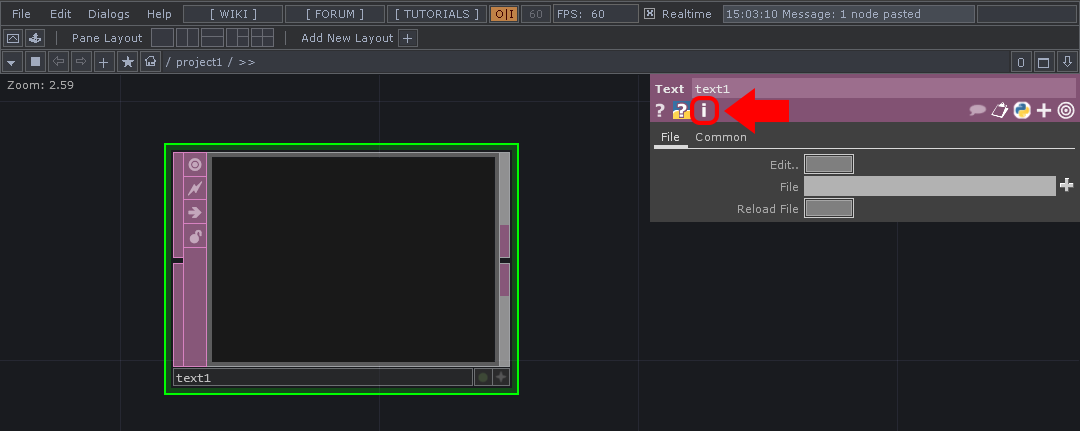
\includegraphics{./img/1.3/navigation-1.png}
\end{center}

Left-click on the 'i' to get more detailed information about the selected operator.

There are several key commands used to navigate TouchDesigner projects. Two of these key commands are 'u' and 'i'. Press 'u' will move up one Network, and out of the current component. To go inside of a Network or component (like a Container COMP or Base COMP), select the component and hit 'i'.

To centralize the screen on all the Operators in a Network, use the 'h' key on the keyboard. This performs the 'Home' action on the current Network. 

\end{fullwidth}

%------------------------------------------------

\section{Networks and Paths}
\begin{fullwidth}
All TouchDesigner projects are made of Networks. A Network is a group of Operators. Networks are encapsulated inside of components, such as a Container COMP, Base COMP, Geometry COMP, etc. Networks can be infinitely nested. The top level is called the 'root' level. TouchDesigner system and UI elements can be found at the 'root' level.

Encapsulating and organizing Networks from the start of the project is a great practice to get in the habit of. The current path is always visible in the 'Path Bar' at the top of the 'Network Editor'.

\begin{center}
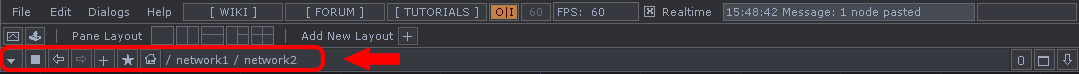
\includegraphics{./img/1.4/path-1.png}
\end{center}

All TouchDesigner Operators have a path. These paths are similar to Unix file paths. There are two kinds of paths to an Operator: the 'absolute path' and the 'relative path'. The 'absolute path' is the path to the Operator from the 'root' of the project, or '/'. The 'relative path' is the path to an Operator from another Operator. These paths start from the Network of the referencing Operator, instead of starting from the 'root'.

Open example 'Paths.toe'. This example demonstrates paths. TouchDesigner will start in the 'root' of the project where there is a Container COMP named 'network1'. Inside of 'network1', there are two Operators. 'rel1' is a Text DAT with two paths in its contents. The first is an 'absolute path'. This path starts from the 'root', or top of the project, and travels towards the Operator. The second path is the 'relative path' from the current Operator to 'rel2', which is a Text DAT inside of the Container COMP named 'network2'. In the 'relative path', the path travels from the current location to the destination. To get from 'rel1' to 'rel2', the path only needs to travel into 'network2', thus the 'relative path' is 'network2/rel2'.

Notice that the viewer of 'network2' is displaying an Operator from inside of it. This technique will be discussed more in later examples, but what is important now is the path used. In the 'Operator Viewer' parameter of 'network2', there is the path to './display', where 'display' is the name of the Operator, and './' denotes one level inside of the referencing Operator, which is 'network2' in this case. 

Inside of 'network2', there is a Text DAT named 'display', whos contents are being displayed in the Network above. The other two Text DATs have more path examples written in them. 'abs1' is another example of an 'absolute path'. 'rel2' has an example of a 'relative path' between itself and 'abs1'. It also has an example of a 'relative path' between itself and 'rel1' in the Network above, where 'rel1' is the Operator's name, and '../' denotes one Network level above the current Network. '../' can be used in sequence to move up as high as the root, but there are more efficient ways of making paths.


\end{fullwidth}

%------------------------------------------------

\section{Using an External Text Editor}
\begin{fullwidth}

Small Python scripts can be created and edited inside of TouchDesigner, but as scripts grow, an external text editor can save a lot of time and trouble.

There are a number of helpful features gained by editing scripts in an external text editor. Without creating an extensive list, some reasons include:

\begin{enumerate}
\item Line numbering 
\item Colour coded syntax
\item Find \& Replace functionality
\item Auto-completion
\end{enumerate}

These features add up to a far richer, and more efficient experience when working extensively with Python inside of TouchDesigner.  

To setup an external editor the steps are as follows:

\begin{enumerate}
\item Open the 'Preferences' dialog found in the 'Edit' menu
\item Go to the 'DATs' preferences
\item Click the file browser icon for the 'Text Editor' setting
\item Assign the the external editor's executable (.exe) by selecting it and clicking 'Open'.  This is usually located in the 'Program Files' folder
\item Click 'Accept' on the Preferences dialog
\end{enumerate}

Once the setup is complete, right click on a DAT and click the 'Edit Contents' option. The DAT will be opened in the program which is specified by this preference.  A separate 'Table Editor' preference is available to set the external editor used for DATs that are tables.

Two well-respected editors that are used frequently in the TouchDesigner community, and are cross-platform, are linked below: 

\begin{description}
\item[Sublime Text 3] \url{http://www.sublimetext.com/}
\item[Notepad++] \url{http://notepad-plus-plus.org/}
\end{description}

\end{fullwidth}
%------------------------------------------------

\section{Help}

\begin{fullwidth}

If there are ever any questions about specific Operators or processes, refer to the official Derivative Wiki. Each Operator has two shortcuts that will open it's Wiki page in a new browser window. These two buttons are located in the Parameter window, and both are represented by question marks. One is specifically about the Operator and it's use, while the other, the question mark over the Python logo, is specifically about Python scripting with that Operator.

\begin{center}
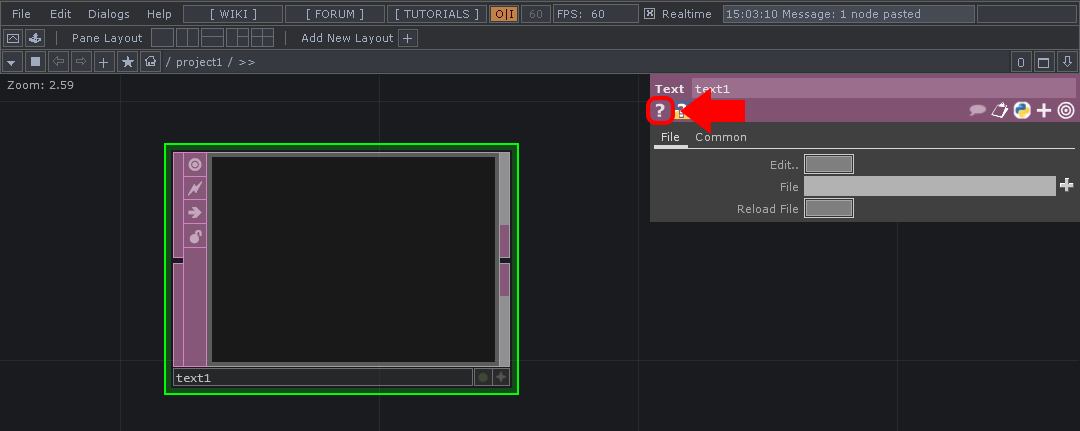
\includegraphics[width=15cm]{./img/1.6/help-1.png}

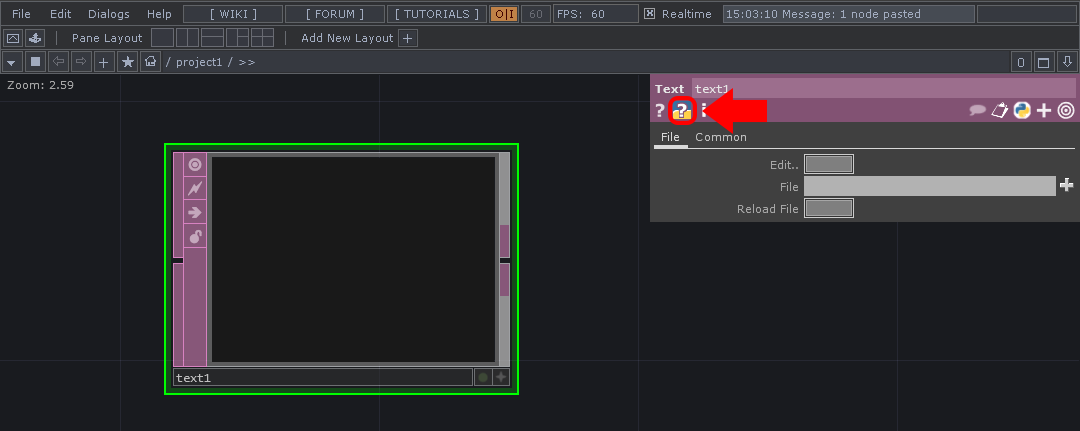
\includegraphics[width=15cm]{./img/1.6/help-2.png}
\end{center}

\end{fullwidth}

%------------------------------------------------

